\documentclass{article}
\usepackage{graphicx}
\usepackage{float}
\usepackage[dvipsnames]{xcolor}
\usepackage{listings}
\usepackage{indentfirst}
\usepackage{paralist}
\usepackage[bookmarks=true]{hyperref}

\lstset{numbers=left,framexleftmargin=10mm,frame=none,backgroundcolor=\color[RGB]{245,245,244},keywordstyle=\bf\color{blue},identifierstyle=\bf,numberstyle=\color[RGB]{0,192,192},commentstyle=\it\color[RGB]{0,96,96},stringstyle=\rmfamily\slshape\color[RGB]{128,0,0},showstringspaces=false}
\begin{document}
\title{\textbf{Design of kdump in the kvmibm-installer}}
\author{Tao Wu}
\date{\today}
\maketitle
%\tableofcontents
\section{Introduction}
Kdump is a kernel crash dumping mechanism and is very reliable because the crash
dump is captured from the context of a freshly booted kernel and not from the
context of the crashed kernel. Kdump uses kexec to boot into a second kernel
whenever system crashes. This second kernel, often called the crash kernel,
boots with very little memory and captures the dump image. \\

The first kernel reserves a section of memory that the second kernel uses to
boot. Kexec enables booting the capture kernel without going through an IPL
sequence, so contents of the first kernel's memory are preserved, which is
essential when kernel crash dump. \\

\section{Introduction of design}

\subsection{Functions provided}
\begin{itemize}
\item Enable or disable kdump mechanism.
\item Automatically or Manually reserve system memory for kdump.
\end{itemize}
\noindent

\subsection{Composition}
The main form consists of
\begin{itemize}
\item A piece of brief introduction text.
\item A check box to enable/disable kdump, enabled by default.
\item A list box providing the choice of `Automatic/Manual' mode of memory
reservation, `Automatic' by default. 
\item An entry for inputting memory size, `128' by default.
\item And a text prompting the size scope which is in the form of [lower,
upper], and lower is 128 by default, while upper is evaluated by running time. 
\end{itemize}
\begin{figure}[H]        
\center{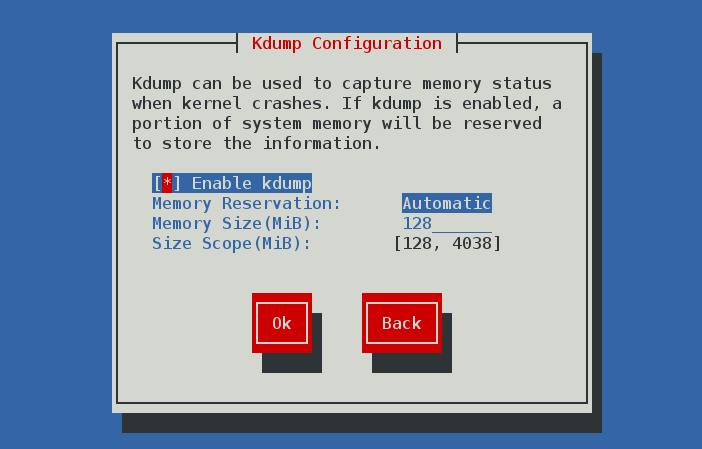
\includegraphics[width=\textwidth]  {k1.png}}        
\end{figure}

\subsection{Navigation}
\subsubsection{Enable/Disable kdump check box}
\noindent
Unselecting the checkbox of ``Enable kdump'' will cause all values being turned to
blank and transferring the focus to the `Ok' button. 
\begin{figure}[H]        
\center{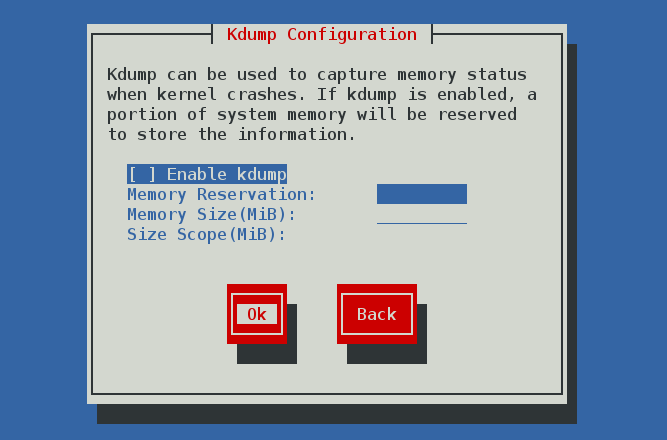
\includegraphics[width=\textwidth]  {k2.png}}        
\end{figure}
\noindent
Alternatively, selecting the checkbox of ``Enable kdump'' will cause all values
being restored to original values and setting the focus at the check box.

\subsubsection{Switch among memory reservation list box}
\noindent
When `Manual' item is selected, the check box of ``Enable kdump'' will be
selected and the memory size entry being opened to accept input, and the
default size scope emerges.\\
\begin{figure}[H]        
\center{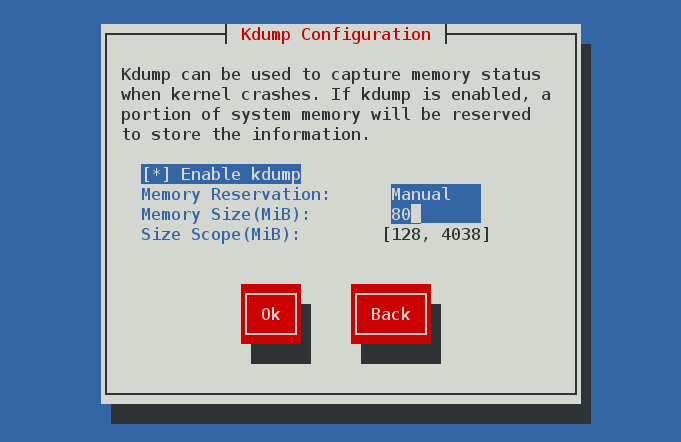
\includegraphics[width=\textwidth]  {k4.png}}        
\end{figure}
\noindent
When `Automatic item is selected, the check box of ``Enable kdump'' will be
selected and the memory size entry changes to `128' and being closed to accept
input, and the default size scope emerges.\\
\begin{figure}[H]        
\center{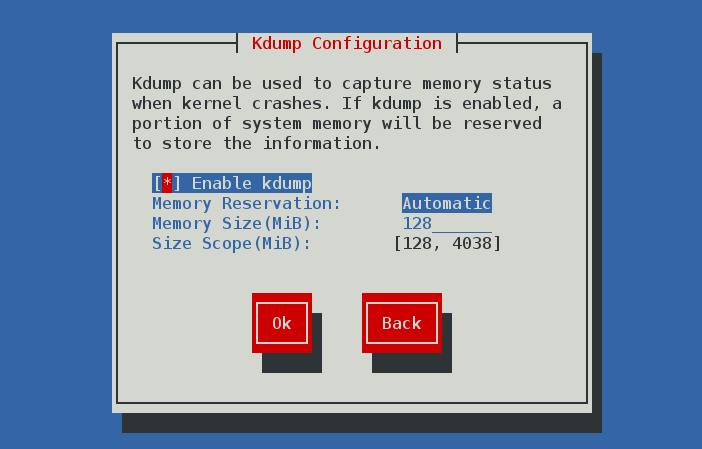
\includegraphics[width=\textwidth]  {k1.png}}        
\end{figure}
\subsubsection{Memory size entry}
\noindent
When the memory reservation list box switches to `Manual' mode, this entry must
be inputted, or an error message box will pop up.\\
\begin{figure}[H]        
\center{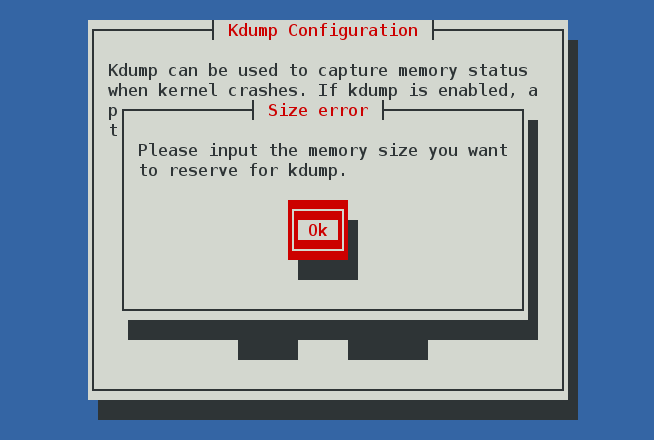
\includegraphics[width=\textwidth]  {k8.png}}        
\end{figure}
\noindent
The value which user inputs needs to be inside the size scope, or an error
message box will pop up.
\begin{figure}[H]        
\center{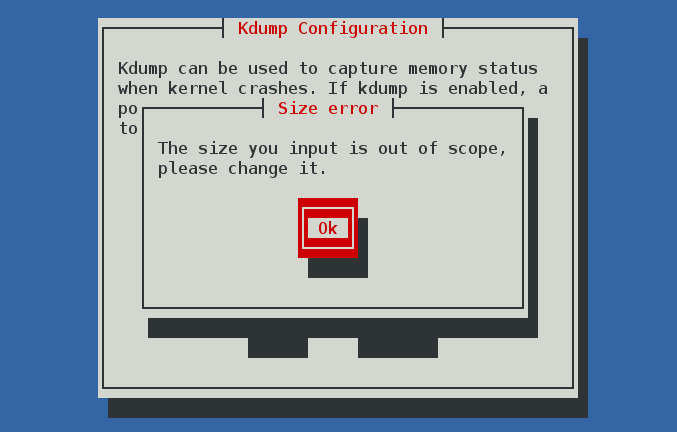
\includegraphics[width=\textwidth]  {k5.png}}        
\end{figure}

\subsection{Help screen}
\noindent
Once 'F3' on the keyboard is pressed, a help screen will pop up.
\begin{figure}[H]        
\center{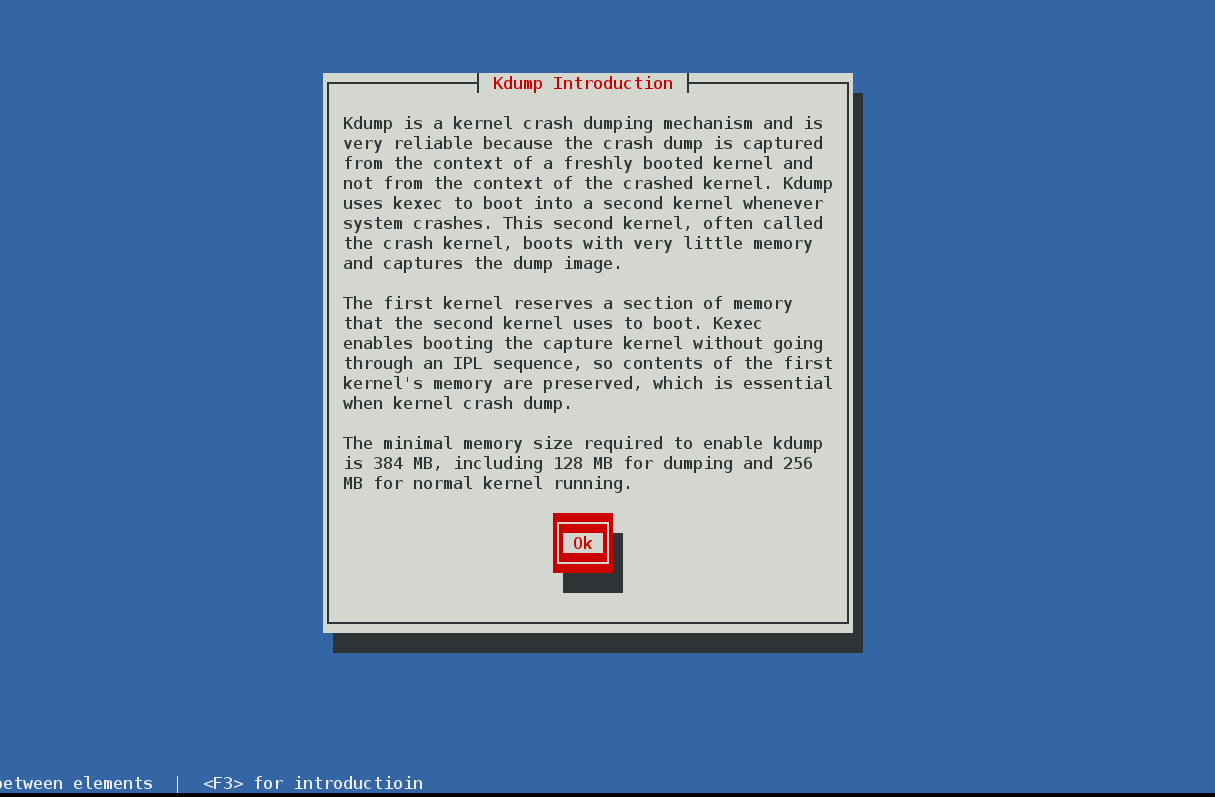
\includegraphics[width=\textwidth]  {k14.png}}        
\end{figure}

\subsection{Deal with insufficient memory}
\noindent
At very rare circumstances, the system possesses less memory than minimal
required size (384 MiB). But if that is the case, the configuration form will be
tailored:\\
1. A piece of prompt text will be added below the introduction text.\\
2. The check box of `Enable kdump' will be unselected, and will be unable to
be selected.\\
\begin{figure}[H]        
\center{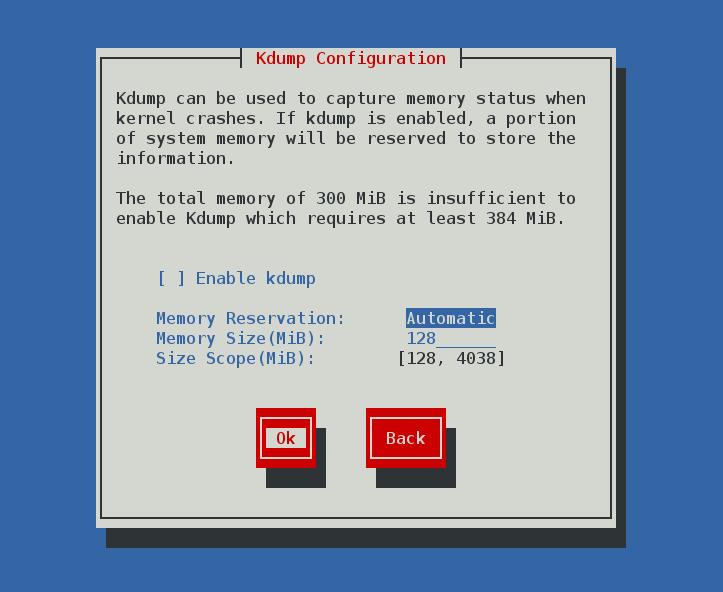
\includegraphics[width=\textwidth]  {k13.png}}        
\end{figure}

\subsection{Reflect in the summary form}
\noindent
1. If the kdump is enabled, the related part of summary form is as:
\begin{figure}[H]        
\center{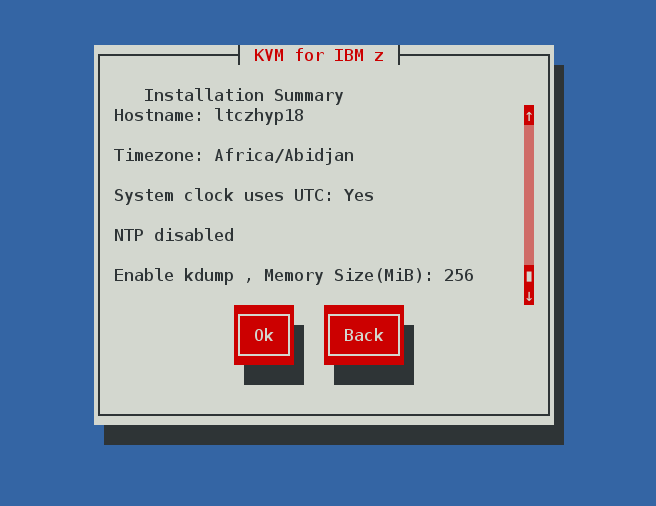
\includegraphics[width=\textwidth]  {k11.png}}        
\end{figure}
2. If the kdump is disabled, the related part of summary form is as:
\begin{figure}[H]        
\center{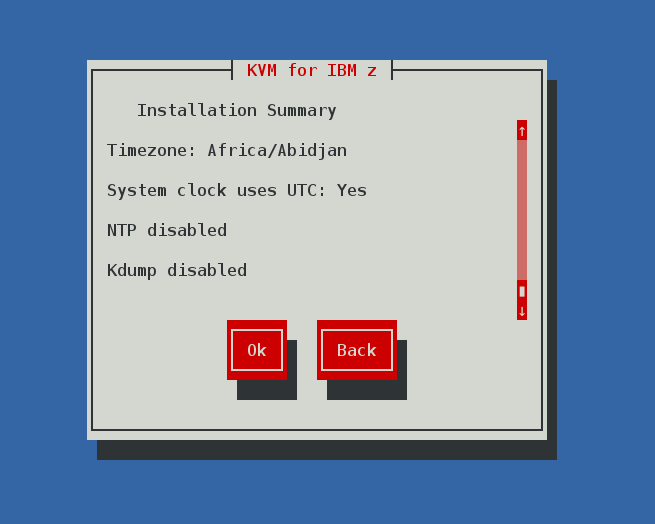
\includegraphics[width=\textwidth]  {k12.png}}        
\end{figure}


\section{Reserved memory size}
\noindent
It is necessary to give a proper memory size scope, and we set this range basing
on:\\

\noindent
A: The minimal memory size required for dumping memory when system crash.
Referring to anaconda, it is 128 MiB.\\
B: The minimal memory size required by system for running kernel and
services. Referring to anaconda, it is 256 MiB.\\
C: The total memory which the system possesses.\\

\noindent
The proper size for kdump is expected to be no less than A and also no more than
C minus B. So the scope of size of kdump should be [128, total memory - 256].
However if C is less than 384(A plus B, 128 + 256) MiB, kdump should not be
enabled.

\section{Capture the Dump}

\noindent
Normally kernel panic() will trigger booting into capture kernel but for testing
purposes one can simulate the trigger in one of the following ways.\\

\begin{itemize}
\item Trigger through /proc interface\\

 \underline{echo c $>$ /proc/sysrq-trigger}\\
\begin{figure}[H]        
\center{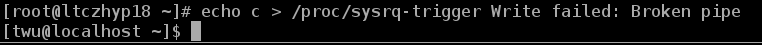
\includegraphics[width=\textwidth]  {crash1.png}}        
\end{figure}

\item Trigger by inserting a module which calls panic()\\
\end{itemize}
\noindent
The system will boot into the capture kernel. A kernel dump will be
automatically saved in /var/crash/$<$dumpdir$>$ and the system will boot back
into the regular kernel. The name of the dump directory will depend on date and
time of crash. For example, /var/crash/127.0.0.1-2015-07-29-09:31:38/vmcore.
Right now we only support local disk (/var/crash) as dump target.\\
\begin{figure}[H]        
\center{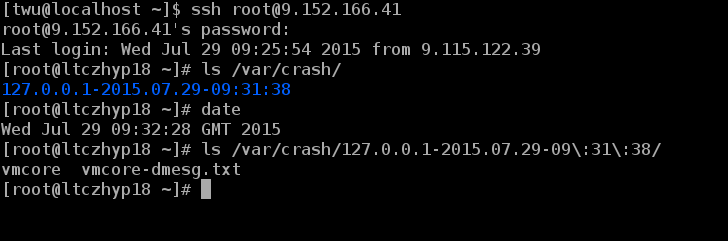
\includegraphics[width=\textwidth]  {crash3.png}}        
\end{figure}
\section{Dump Analysis}

\noindent
Once the system has returned from recovering the crash, you may wish to analyse
the kernel dump file using the crash tool.\\

\begin{itemize}
\item First, locate the recent vmcore dump file:\\

  \underline{find /var/crash -type f -mtime -1}\\

\item Once you have located a vmcore dump file, call crash:\\

\end{itemize}
\underline{crash /var/crash/127.0.0.1-2015-07-29-09:31:38/vmcore /usr/lib/debug/lib/modules/`uname -r'/vmlinux}
\begin{figure}[H]        
\center{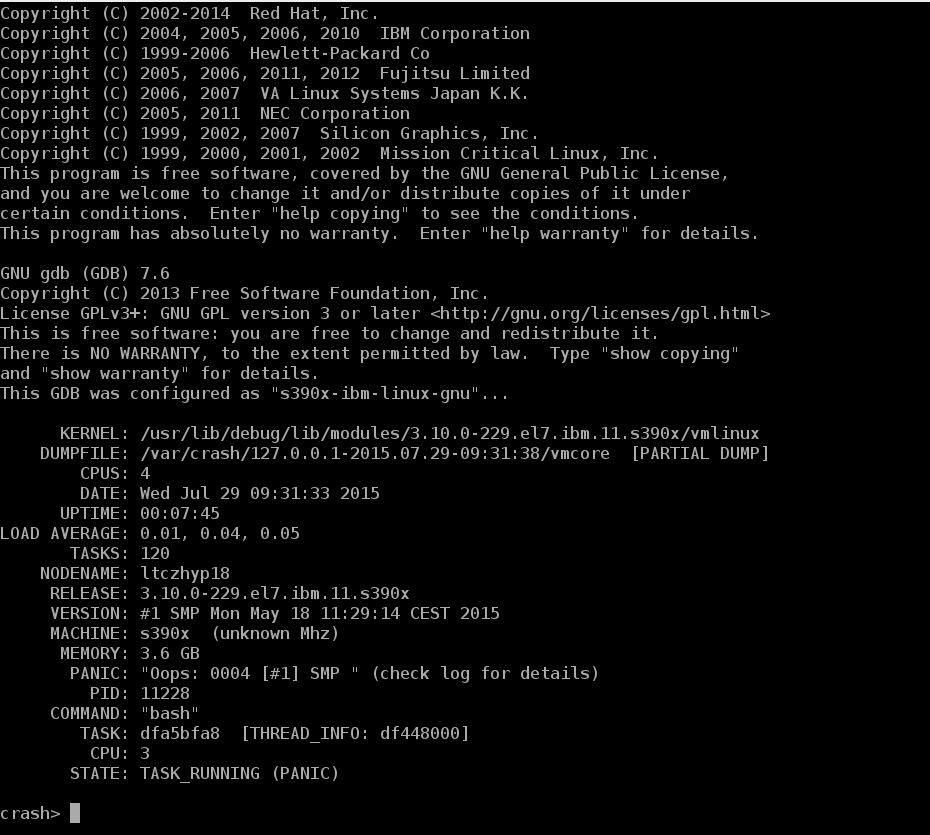
\includegraphics[width=\textwidth]  {crash4.png}}        
\end{figure}
\end{document}
